\chapter{Analysis overview}
\label{ref:overview}

This analysis aims at the measurement of \RD and \RDst,
with the definition reproduced from the introduction:
\begin{equation}
    \RDX \equiv \frac{\BFDTau}{\BFDMu}
\end{equation}
from LHCb 2016 data\footnote{
    It is planned to use full LHCb run 2 data (2016--2018) at a later date.
}, reconstructed in (with visible final state particles marked in red):
%%%%
\begin{itemize}
    \item $\Bzb \rightarrow \Dstarp (\rightarrow \Dz (\rightarrow \textcolor{red}{\Km \pip})\textcolor{red}{\pip}) \taum (\rightarrow \textcolor{red}{\mun} \neumb \neut) \neutb)$
        for \RDst signal decay\footnote{
            A parton level diagram for the signal decays is drawn in
            \cref{fig:decay-diagrams} as a reference.
        }
    \item $\Bzb \rightarrow \Dstarp (\rightarrow \Dz (\rightarrow \textcolor{red}{\Km \pip})\textcolor{red}{\pip}) \textcolor{red}{\mun} \neumb$
        for \RDst normalization decay
    \item $\Bm \rightarrow \Dz (\rightarrow \textcolor{red}{\Km \pip}) \taum (\rightarrow \textcolor{red}{\mun} \neumb \neut) \neutb)$
        for \RD signal decay
    \item $\Bm \rightarrow \Dz (\rightarrow \textcolor{red}{\Km \pip}) \textcolor{red}{\mun} \neumb$
        for \RD normalization decay
\end{itemize}
such that $\Dstarp\mun$ and $\Dz\mun$ are the final reconstructed states
which are often referred in this text as \Dstar channel and \Dz channel in later
chapters.
These states are chosen so that the final state particles
(e.g. $K^-, \pi^+, \mu^-$) are all charged,
because the LHCb detector is not well-suited for neutral particle
reconstruction.

\begin{figure}[!htb]
    \centering
    \resizebox{0.8\textwidth}{!}{
        \begin{tikzpicture} \begin{feynman}
    \vertex (a1) {\(b\)};
    \vertex[right=7em of a1] (a2);
    \vertex[right=7em of a2] (a4) {\(c\)};

    \vertex[below=3em of a1] (b1) {\(\overline q\)};
    \vertex[below=3em of a4] (b2) {\(\overline q\)};

    \vertex at ($(a2)!0.5!(a2)!0.5cm!90:(a2)$) (d);

    \vertex[right=7em of a4] (e1) {\(\nu_\tau\)};
    \vertex[above right=3em of e1] (e2);
    \vertex[below right=of e2] (e3) {\(\mu^-\)};
    \vertex[above right=of e2] (e4) {\(\overline\nu_\mu\)};

    \vertex[above=3em of a4] (c2);
    \vertex at ($(c2)!0.5!(e1)$) (c1);
    \vertex[above right=3em of c2] (c3) {\(\nu_\tau\)};

    \diagram* {
        (a1) -- [fermion] (a2) -- [fermion] (a4),
        (b2) -- [fermion] (b1),
        (c3) -- [fermion] (c2) -- [fermion, edge label=\(\tau^-\)] (c1),
        (a2) -- [blue, boson, edge label=\(W^{-}\)] (c2),
        (c1) -- [fermion] (e1),
        (c1) -- [boson, edge label=\(W^-\)] (e2),
        (e2) -- [fermion] (e3),
        (e2) -- [anti fermion] (e4),
    };

    \draw [decoration={brace}, decorate] (b1.south west) -- (a1.north west)
        node [pos=0.5, left] {\(B\)};
    \draw [decoration={brace}, decorate] (a4.north east) -- (b2.south east)
        node [pos=0.5, right] {\(D^{(\ast)}\)};
\end{feynman} \end{tikzpicture}

    }

    \caption{
        Parton level diagrams for $B \rightarrow D^{(*)} \taum\neutb$ signal
        decays,
        where $\overline q$ can be either a $\overline u$ or a $\overline d$.
    }
    \label{fig:decay-diagrams}
\end{figure}


\paragraphtoc{Feed down}
A complication of these states is that they are \emph{inhomogeneous},
that is, not all \Dz\mun final state events are actual decays with just \Dz\mun
in their final states:
some $\Bzb \rightarrow \Dstarp\ellm\neulb$ decays feed down into the \Dz\mun
states,
because \Dstarp decays strongly to a \Dz and a slow \pip,
with the latter often missed in the reconstruction;
for example, a slow \pip with a momentum\footnote{
    The mean momentum of a slow \pip is around 8~GeV.
    Generally a lower momentum implies a lower track finding efficiency.
} of 10~GeV will fail to register a
well-defined track in the detector about 35\% of time,
% Source:
%   https://indico.cern.ch/event/719661/contributions/3115144/attachments/1707415/2751519/WGprod_TurVal_Renata.pdf
%   p. 7, Long method
thus no \Dstarp is constructed for this event.
In addition, $\Bm \rightarrow \Dstarz\ellm\neulb$ decays,
which have a branching fraction of about 2.5 times larger compared to
$\Bm \rightarrow \Dz\ellm\neulb$ decays,
contribute exclusively to \Dz\mun states, because the neutral slow
\piz, a product of the \Dstarz decay, is entirely missed.
Therefore, a \emph{simultaneous} fit,
assuming isospin symmetry,
to both \Dstarp\mun and \Dz\mun states is needed to
account for the correlations between \RD and \RDst and improve the
precision\footnote{
    As opposed to extracting \RDst from the \Dstarp\mun sample alone.
} of \RDst.


\paragraphtoc{Background contributions}
In addition to the signal, normalization, and feed down from \Dstar modes,
both \Dstarp\mun and \Dz\mun final states contain contributions from many
background decay modes that are only partially reconstructed,
which can be categorized as follows:
\begin{itemize}
    \item Four $1P$ \Dstst:
        these are the lightest excited $D$ mesons.
        These \Dstst states decay in a cascade manner:
        $B \rightarrow \Dstst
        (\rightarrow D^{0|*|**} (\rightarrow D^{0|*}\pi) \pi)
        l\neul$,
        contributing to both \Dz and \Dstar channel with additional
        charged or neutral pions in the final states.
    \item Highly excited \Dstst (\Dstst heavy, $\Dstst_H$):
        these refers to the excited $D$ mesons that are heavier than the four
        $1P$ \Dstst states.
        The predicted masses of
        the known $D$ mesons, including \Dz, \Dstar, the four $1P$ \Dstst,
        and highly excited \Dstst,
        are displayed in \cref{fig:excited-d-meson}.
        Similar to the four $1P$ \Dstst states,
        the \Dstst heavy states cascade decay into a \Dz or a \Dstar,
        with two or more extra pions in the final states:
        $B \rightarrow \Dstst_H (\rightarrow D^{0|*} \pi\pi) \mu\neum$.

\begin{figure}[!htb]
    \centering
    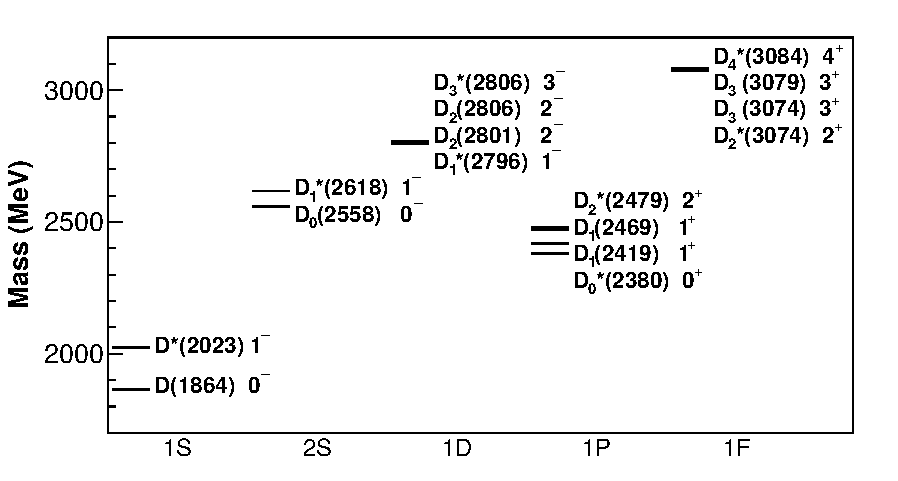
\includegraphics[width=0.7\textwidth]{figs-analysis-overview/d_meson_predicted_masses.pdf}
    \caption{
        Modified Godfrey-Isgur mass predictions for $D$ mesons.
        Taken from \cite{D_mesons_2013}.
    }
    \label{fig:excited-d-meson}
\end{figure}

    \item \DststS:
        the $B_s \rightarrow (D'_{s1}|D_{s2})
        (\rightarrow D^{(*)}K) l\neul$
        decays have one extra kaon in their final states.
    \item $DDX$:
        the double-charm backgrounds,
        namely $B \rightarrow D^{(*)} D_q X$ decays
        where $D_q$ stands for a generic charm meson with $q$ being a
        $u/d/s$ quark and $X$ represents extra pion(s), a kaon, or an
        excited $K$ states.
        The lepton in such decays comes from
        a leptonic (when $q = s$) or a semileptonic
        (when $q = u \text{ or } d$) decay of the $D_q$.
        These decays contain many additional final state particles with at least
        one kaon.
\end{itemize}

The backgrounds due to \emph{mis-reconstructions} of the \DXmu pair must
also be taken into account, namely:
\begin{itemize}
    \item Muon misID:
        sometimes the \muon in the \DXmu pair is mis-identified
        because the particle identification algorithm is not 100\% accurate.
        When such misidentification happens,
        the ``\muon'' can be a pion, a kaon, a proton, an electron,
        or a ghost\footnote{
            Fake tracks due to random combinations of track segments, a detector
            effect.
        }.
    \item Combinatorial backgrounds:
        these refer to random combinations of the \Dz \muon
        (for the \Dz channel),
        \Dstar \muon, or \Dz \pion (the latter two are for the \Dstar channel)
        that do not originate from the decay of the same $B$ meson.
\end{itemize}


\paragraphtoc{Signal and control skims}
The \DXmu pairs are selected such that they are likely coming from
the same $B$ decays.
However such selection criteria does not take the extra track(s) in the events
from the background decays into account.
The selected \DXmu samples are further split into signal-enriched and
background-enriched sub-samples, named as ``skims'',
based on the isolation property of the \DXmu pair,
that is, how likely that other well-reconstructed tracks in the same event
are originating from the same $B$ as the \DXmu.
There are four resulting skims, namely:
\begin{itemize}
    \item ISO:
        signal-enriched. The \DXmu pair is well-isolated as there
        is no other track in the event that is likely coming from the same $B$.
    \item 1OS:
        enriched in $B \rightarrow \Dstst \ellm\neulb$.
        The 1OS skim contains events with one extra pion that is originating
        from the same $B$ as the \DXmu pair
        (anti-isolated).
    \item 2OS:
        enriched in $B \rightarrow \Dstst_H \mun\neumb$.
        Contain events with two anti-isolated pions.
    \item DD:
        enriched in $B \rightarrow D^{(*)} D_q X$.
        Contain events with one or more anti-isolated tracks with one
        of them being a kaon.
\end{itemize}


\paragraphtoc{Fit overview}
The signal, normalization, and backgrounds all have differing kinematics
which are for the most part modeled from Monte-Carlo simulation (MC),
and sometimes from data control samples.
These differences are used in the fit to determine the yields of all
relevant decay modes.
The differentiating kinematic variables, defined in the \B rest frame,
referred as ``fit variables'',
are the following:
%%%%
\begin{itemize}
    \item \mmSq: Defined as $(p_B - p_{D^{(*)}} - p_\mu)^2$,
        the missing mass (squared) is typically due to missing (unreconstructed)
        neutrino(s).
        For $B \rightarrow D \mun \neumb$ decays, only 1 neutrino is missing,
        so \mmSq is small ($\sim$ the mass of neutrino);
        for $B \rightarrow D \taum (\rightarrow \mun\neumb\neut) \neutb$,
        3 neutrinos are missing, and \mmSq can be large.
    \item \el: The energy of \mun in the $B$ rest frame.
        \mun coming from \taum decays are typically
        softer, i.e. with smaller energy, due to reduced available phase space.
    \item \qSq: The momentum transfer, defined as the invariant mass squared
        of the virtual $W$ boson (marked in blue in \cref{fig:decay-diagrams})
        and calculated as $(p_B - p_{D^{(*)}})^2$.
        The \qSq spectra of
        $B \rightarrow \text{P} \ell\neu$ and $B \rightarrow \text{V} \ell\neu$
        decays are notably different,
        where ``P'' stands for a pseudoscalar meson (e.g. \Dz),
        and ``V'' a vector (e.g. \Dstar);
        the \qSq spectrum is softer
        (more likely to be at lower \qSq) for pseudoscalar mesons.
        In addition, the semitauonic decays are restricted to the phase space
        where $\qSq > m^2_\tau$,
        whereas the semimuonic decays extend down to $\qSq > m^2_\mu \approx 0$.
        Both modes share a common \qSq upper bound $(m_B - m_{D^{(*)}})^2$
        where the $D$ meson is produced at rest in the $B$ rest frame.
\end{itemize}
%%%%
These variables, however, cannot be deduced exactly at LHCb:
because \B mesons
are typically produced from hadronization of $pp$ collisions,
carrying an unknown portion of $pp$ momenta,
the \B momentum and its rest frame are not known.
A procedure, termed ``rest frame approximation'' (RFA), is developed for LHCb
to estimate the \B rest frame, making computation of fit variables possible.
% As an demonstration that RFA can reproduce these variables reasonably well,
% MC true rest frame variables and estimated variables with RFA for
% $\Bm \rightarrow \Dz\mun\neumb$ decay are shown in
% \cref{fig:rfa-variables}.
More information about RFA can be found in \cref{appx:rfa}.

% \begin{figure}[!htb]
%     \caption{
%         MC true rest frame variables vs. estimated variables with RFA in
%         $\Bm \rightarrow \Dz\mun\neumb$ decay.
%     }
%     \label{fig:rfa-variables}
% \end{figure}

This analysis uses the same general fit strategy in the LHCb \RDX run 1
analysis:
fit the parameters characterizing various background decays with separate
\emph{control skims} (1OS, 2OS, and DD),
then import these parameters either as constraints or fully fixed into the
signal fit;
this is because while the \emph{signal skim} (ISO) contains many
backgrounds,
they are only a small fraction relative to the signal and normalization
combined,
thus no good description of the backgrounds can be extracted from the signal fit
alone.


\paragraphtoc{Workflow}
%%%%
As an update to the previous analysis, this analysis shares a similar
workflow with that of run 1.
The workflow of this analysis is:
First, \Dstarp\mun and \Dz\mun final states are selected with the procedure
described in \cref{ref:sel}.
Then, emulation of certain detector responses to MC are carried out offline
with the procedure described in
\cref{ref:mc-emulation},
as this analysis requires a large number of simulated events with only partial
detector simulation to be computationally viable.
Afterwards, various mis-modelings in the MC simulation,
mainly in form factor modeling and detector response, are updated and
corrected with the procedures detailed in \cref{ref:mc-cor}.
Finally, \RDX are extracted from a simultaneous fit described in \cref{ref:fit}.
The estimation of major systematic uncertainties is discussed in
\cref{ref:sys-uncert}.


\paragraphtoc{Differences between the run 2 and run 1 analyses}
The major differences between this analysis and the pathfinder run 1 \RDX
analysis are:
\begin{itemize}
    \item Due to a larger integrated luminosity
        (5.4~fb$^{-1}$ in run 2 versus 3.1~fb$^{-1}$ in run 1),
        a larger $B$ production cross section due to higher collision energy
        (13~TeV center of mass energy in run 2 versus 7~TeV in run 1),
        and a dedicated trigger resulting in a higher selection efficiency,
        the run 2 analysis can work with a much larger dataset:
        for 2016 alone (1.6~fb$^{-1}$),
        the selected \Dz\mun signal sample contains 2,178,793 events,
        whereas for run 1 combined (3.1~fb$^{-1}$) 1,734,133 events,
        a factor of $\sim\!1.26$ gain.

        As briefly mentioned before,
        a large amount of MC is needed to control the total statistical
        uncertainties,
        which makes it impractical to simulate most of the detector.
        Instead, only the tracking system is simulated and additional detector
        responses such as hardware triggers are \emph{emulated} offline.

    \item In order to update (reweight) MC form factor models offline,
        the run 1 analysis implemented two ad-hoc approaches for form factor
        reweighting:
        one is based on \texttt{XslFF} reweighting class from BaBar,
        the other is completely in-house.
        A large amount of time is spent on validation of the form factor
        reweighting implementations.

        Recently, a new software package, named \Hammer, allows easier form
        factor reweighting and comes pre-validated by the \Hammer authors.
        This analysis leverages on \Hammer for an easier to implement and more
        reliable form factor reweighting procedure.
\end{itemize}


% Additional information is organized as follows:
% An overview of theory of semileptonic \B decay is provided in
% \cref{ref:theory},
% followed by a brief introduction to the LHCb detector in \cref{ref:detector}.
% The ``conclusion'' of this still ongoing analysis is provided in
% \cref{ref:conclusion}.
